
\documentclass{ctexart}

\author{李约瀚 \\ 14130140331 \\ qinka@live.com \\ qinka@qinka.pw}
\title{KWIC 翻译}
\usepackage{listings}

\begin{document}
\maketitle

\section{功能性需求}

在 1974年, Parnas 提出了如下问题:
\begin{itemize}
    \item 接受一行有序的输入
    \item 一行输入由若干词汇组成
    \item 每个单词用若干字母组成
    \item 任何一行可以进行循环移位:将行首单词移至行尾
    \item KWIC 索引系统输出一个按字母顺序排列的循环移位的全排列
\end{itemize}

\section{非功能性需求}

\subsection{可修改性}
\begin{itemize}
    \item 算法的更改
    \item 数据表现方式改变
    \item 系统功能扩展
\end{itemize}

\subsection{性能}
\begin{itemize}
    \item 时间空间复杂度
\end{itemize}
\subsection{重用性}
\begin{itemize}
    \item 系统的部分组成内容(服务)是可重用组件
\end{itemize}

\section{主程序/子过程}

主程序/子过程的方式就是简单的将问题根据基本的四个要求分解成:输入、以为、分组与输出。
这些组件由主函数按照一定的顺序作为子过程进行调用控制。
数据则通过一个不受约束的共享储存的协议在组件之间传递。
\begin{figure}[h!]
\centering
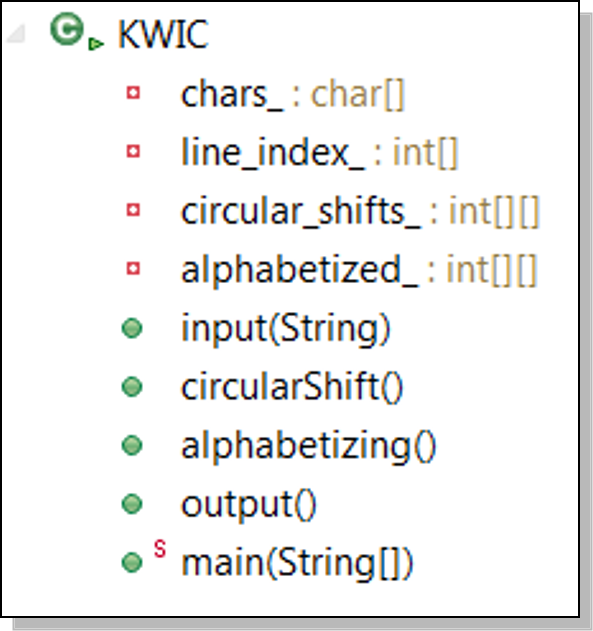
\includegraphics[width=0.7\linewidth]{homework1-shared_data}
\caption{主函数/子过程的结构}
\label{fig:homework1-shared_data}
\end{figure}
\subsection{调用过程}

输入函数被调用用于输入与解析输入的每一行。然后将这些数据表示用字符与对应的行索引。
主函数调用 \lstinline|circularShift| 函数来进行循环移位操作,作用于每一行的数据。然后再将这些数据储存成循环位移数组。
主函数之后调用 \lstinline|alphabetize| 函数将循环位移数组中的结果按照拉丁文字母表的顺序进行排序。然后输出成有序数组。
最后调用 \lstinline|output| 函数将结果输出。

\begin{figure}[h!]
    \centering
    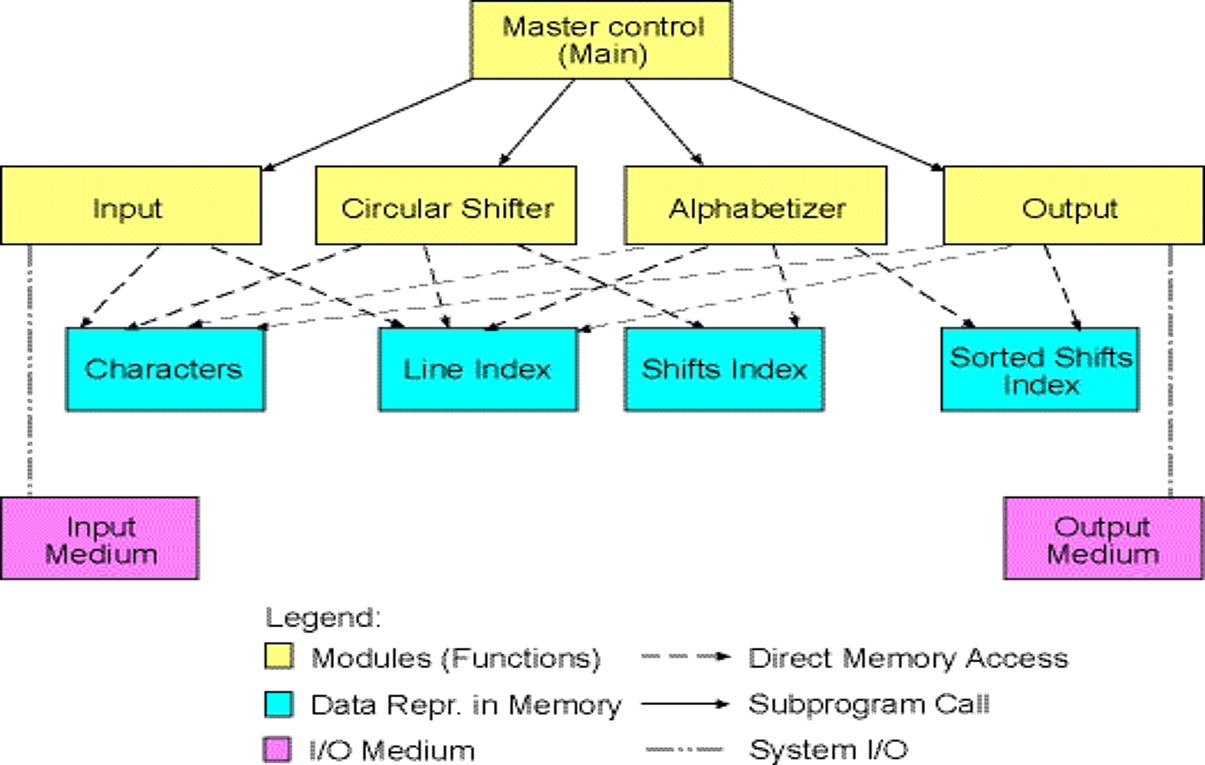
\includegraphics[width=0.7\linewidth]{homework1-shared_data2}
    \caption{调用结构图}
    \label{fig:homework1-shared_data2}
\end{figure}


\subsection{优点}
数据可以被有效的表示出来,特别是计算就算结果可以被同样的储存结构共享。

不同的计算方式在不同的模块中是独立的。

\subsection{缺点}
改变一处数据的ABI或者数据格式,会影响全部模块。

对算法与增加系统功能不容易实现。

这种分解不容易支持重用。

\section{面向对象}
采用面向对象的思想,将数据与作用在数据的读写操作封装在类中,主程序调用这些类生成的实例,形成控制流。
数据不在直接组件之间共享,公用。每个模块提供了一个接口以便其他模块通过接口访问数据,并进行操作。

\begin{figure}[h!]
  \centering
  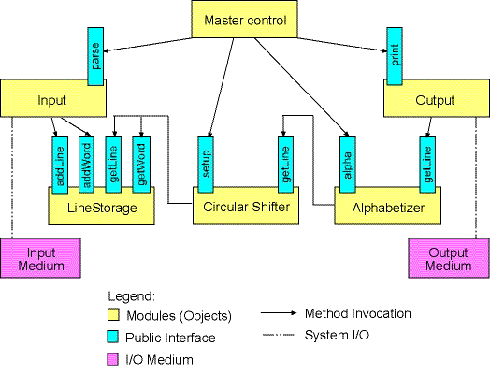
\includegraphics[width=0.7\linewidth]{homework1-oo-1}
  \caption{OO关系}
  \label{fig:homework1-oo-1}
\end{figure}

\subsection{组件分工}
\begin{table}[h!]
  \centering
  \caption{组件分工}
  \begin{tabular}{c|c}
    \verb|Input OBJECT| & 负责从输入读取数据并存储至 \lstinline|LineStorage| 中\\
    \verb|LineStorage OBJECT| & 负责处理字符、单词、行\\
    \verb|CircularShifter OBJECT| & 负责对 \lstinline|LineStorage| 对象中的数据进行循环位移 \\
    \verb|Alphabetizer OBJECT| & 负责对循环位移得到的结果进行排序处理\\
    \verb|Output OBJECT| & 负责答应输出 \\
    \verb|Master Control OBJECT| & 负责空着体罚对象中调用的次序 \\
  \end{tabular}
\end{table}


\subsection{优点}

算法与数据表示可以被独立的更改,而不会影响其他模块。
重用被更好的支持了,模块使得相互作用的不确定性减少。

\subsection{缺点}

设计无法良好的适应新增的功能或者其他的内容。
添加新功能时影响类与模块,同时添加新模块不是十分方便,而过多的调用影响性能。


\section{比较}
面向对象相对要好于主程序/子过程要更优。依赖耦合相对较少,设计易于使用、维护、复用等。

\end{document}